\chapter{準備}
本章では,Python言語の概要,本研究で使用したPython言語のライブラリ,及び, 株の基本知識と株取引で使われているテクニカル分析の指標について述べる.
\section{株について}
本節では,株に関する基礎知識と専門用語について簡単に説明する.
\subsection{株}
株とは企業が資金調達して事業行うために発行しているものである.株を買って保有することで出資者となり,会社のオーナーの一人になることができる\cite{stock}.

\subsection{株価}
株価とは,株式市場において売買が成立したときの株の価格のことである\cite{pythontrading}.
\subsection{株価データ}
株価データとはある一定期間の株価の始値,高値,終値をまとめたものである.期間は分,日,週,月,年等がある.短期の株価を参照する場合は3分,5分などの分単位,長期的な場合は週や月単位の株価データを用いる.
よく使われているのは日単位が多く,本研究も日単位を用いる\cite{pythontrading}.
\subsection{株価チャート}
株価チャートとは株価データをグラフ化し,見やすくしたものである.主に移動平均線とローソク足チャートが取引に使われている\cite{pythontrading}.

\subsection{移動平均線}
移動平均線とは,一定期間の株価の終値より平均値を計算し,その値を元に折れ線グラフで表したものである.
毎日の株価の平均を計算するため,平均値が移動していくことから移動平均またはMoving average(MA)と呼ばれる.

$n$日間の移動平均線のことを$n$日移動平均線と呼ぶ\cite{pythontrading}.本論文では提案アルゴリズムにおいて60日移動平均線を用いる.

\subsection{ローソク足チャート}
ローソク足とは,一定時間内の始値,高値,安値,終値を一本の蝋燭型のグラフに表したものである.終値が始値より高い場合を
株価分析ではローソク足が用いられることが多い.本論文では,株価チャートとして用いる\cite{pythontrading}.

\begin{figure}[H]
  \centering
  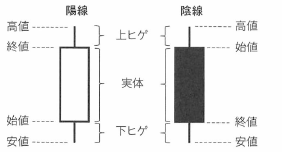
\includegraphics[width=110mm]{fig/candle.png}
  \caption{ローソク足(引用元\cite{pythontrading})}
  \label{fig:candle}
 \end{figure}

 \subsection{日経平均株価}
日経平均株価とは,日本経済新聞社が東京証券取引所プライム市場上場銘柄から選定した225銘柄の株価の平均ことである\cite{nikkei_kabu}.

 \subsection{利益確定}
 利益確定とは,買った株の値段が上がったときに売却し,利益を確定することである.「利食い売り」ともいわれる.ある程度利益を確定して売却することで損失に転換するリスクを可能性を回避できる\cite{rikaku}.
 \subsection{損切り}
損切りとは,損失を抱えている状態で抱えている株を売却して損失を確定させることである.ロスカットやストップロスなどとも呼ばれている.価格が下落し続けている株を保有しておくと損害が大きくなるため,損切りで損失額を抑えることができる\cite{songiri}.
\section{テクニカル指標}
\subsection{MACD(Moving Average Convergence and Divergence)}
% MACD(Moving average Convergence and Divergence)とは短期の移動平均線が中期の移動平均線を下から上に突き抜け,
% かつどちらも横ばいまたは上向きの状態で買いのタイミングとされているゴールデンクロスをもう少し汎用的にしたテクニカル指標のことである.
% MACDでは移動平均が単純移動平均ではなく,直近の価格になるほど比重をおいて計算する平滑移動平均を用いている.
短期と中期の移動平均線がどちらも横ばいか上向きで
あり,短期移動平均線を中期移動平均線が下から上に
突き抜ける買いのタイミングをゴールデンクロスと呼
ぶ.MACD\cite{pythontrading}は,1970年代後半に米国のシグナラート・コーポレーション社の経営者であったジェラルド・アペル氏によって考案された指標であり,
このゴールデンクロスを更に汎用的に
したテクニカル指標である.MACD では移動平均とし
て,単純移動平均ではなく,直近の価格に比重をおく
平滑移動平均を用いる.
MACDは以下の3つの要素で構成されており,各要素の求め方は以下の通りである.
\begin{itemize}
  \item MACD線=X期間の短期移動平均線(EMA) ‐ Y期間の長期移動平均線(EMA)
  \item シグナル線=MACDのZ期間の単純移動平均線(EMA)
  \item ヒストグラム(OSCI)=MACD線 - シグナル線
\end{itemize}
X,Y,Zはパラメータで,本研究ではX=5,Y=20,Z=9を用いる.MACDとシグナルは折れ線グラフで表し,ヒストグラムは棒グラフで表す\cite{pythontrading}.MACDの買いシグナルは,MACD線がシグナル線を下から上に
突き抜ける場合で,売りシグナルは,シグナル線がMACD線を下から上に
突き抜ける場合である.

図\ref{fig:macdex}でMACDの例を示す.この図ではMACDのMACD線,シグナル線,ヒストグラムが示されている.
MACD線がシグナル線が上から下に突き抜けた時に売りシグナルが出ており,売りのタイミングであることがわかる.
同様に,MACD線がシグナル線を下から上に突き抜けたときにシグナルが出ており,買いのタイミングであることがわかる.
ヒストグラムは,売りシグナルのとき正から負になっており,買いシグナルのときは負から正になっていることがわかる.
\begin{figure}[H]
  \centering
  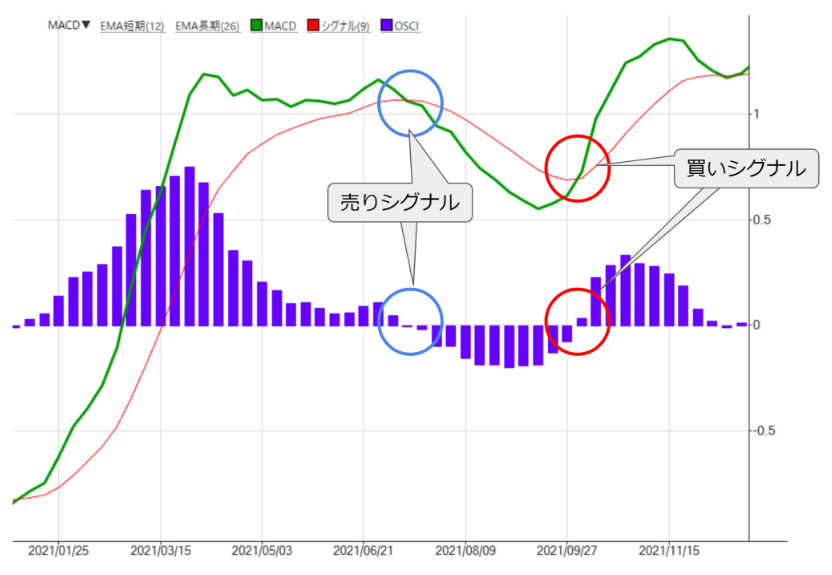
\includegraphics[width=110mm]{fig/macd_exp.png}
  \caption{MACDグラフ(引用元\cite{macdexp})}
  \label{fig:macdex}
 \end{figure}


\subsection{ボリンジャーバンド (BB: Bollinger Band)}
ボリンジャーバンド\cite{pythontrading}とは移動平均線の上下に標準偏差を元に計算された3つのバンドという線を用いるテクニカル指標である.
ボリンジャーバンドの定義式は以下のようになる.
\begin{itemize}
  \item 中央のバンド = $n$日の移動平均線
  \item 上部バンド = 中央のバンド + ($n$日の標準偏差 × X)
  \item 下部バンド = 中央のバンド - ($n$日の標準偏差 × X)
\end{itemize}
nは期間のことであり,本研究では25日を用いている.Xは標準偏差の倍数で1から3までであり,単位はσで扱う.バンドは+1σ (アッパーバンド1), +2σ (アッパーバンド2), +3σ (アッパーバンド3),
-1σ (ロワーバンド1),-2σ (ロワーバンド2), -3σ (ロワーバンド3)の名前で扱う.
株価の変動はバンドの範囲内に収まることが多いと考えられており,ばらつきが多いほど標準偏差は大きくなるため,バンドの幅が広くなる方に値動きが大きくなると判断できる.
株価が収まる確率は以下の通りだとされている\cite{pythontrading}.
\begin{itemize}
  \item ±1σ:68.2%
  \item ±2σ:95.4%
  \item ±3σ:99.7%
\end{itemize}
BBはローソク足とともに表示されることが多く,ローソク足の位置で株価の上がり下がりの余地がどれくらいあるかを判断する.
±3σは±2σとの差が4%しかないため指標としてはあまり重視されない.本論でも±2σをつかって検証する.

図\ref{fig:bbex}はBBの例を示している.移動平均線を基準に±3σ,±2σ,±1σのバンドを示している.BBの買い売りシグナルはいくつかあるが本論では,終値が‐2σを下回ったときに買いシグナルを出すアルゴリズムを提案している.

\begin{figure}[H]
  \centering
  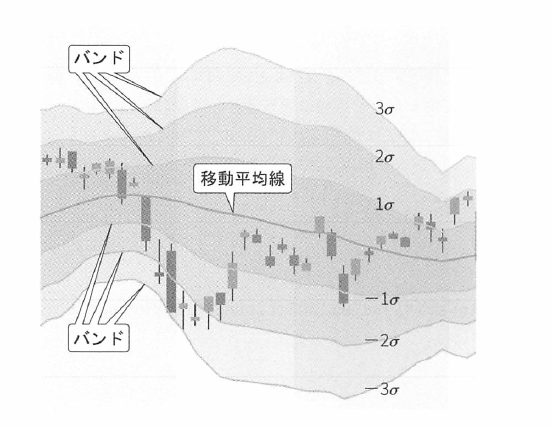
\includegraphics[width=110mm]{fig/bbexp.png}
  \caption{BBグラフ(引用元\cite{pythontrading})}
  \label{fig:bbex}
 \end{figure}
\section{Pythonによるバックテスト環境}

\subsection{Pythonの概要}
% Pythonはオープンソースのインタプリタのオブジェクト指向プログラミング言語で,構文は読みやすく,ライブラリも豊富なため
% 初心者に向いている.コンパイルのステップがないため,編集,テスト,デバッグのサイクルが早い.
% 主な使われている用途としてウェブアプリ,科学的、数値計算,デスクトップGUIで使われている.\cite{pythonapp}
Python\cite{pythontrading,pythonapp,van}は高水準のプログラミング言語であり,直感的で読みやすい構文を持つことが特徴である.1991年にGuido van Rossumによって設計され,その後コミュニティによって発展していった.Pythonは汎用性が高く,ウェブ開発,データ解析,機械学習,人工知能などさまざまな分野で広く利用されている.

Pythonの特徴的な構文として,インデント(行頭の空白文字)を使ったブロック構造があり,これにより可読性が向上し,他のプログラミング言語よりもコードが書きやすい.また,動的型付けを採用しており,変数の型を事前に宣言する必要がないため柔軟性がある.
標準ライブラリが豊富であり,多くの便利なモジュールが組み込まれている.これにより,ファイル操作,ネットワーク通信,データ処理などの様々なタスクを容易に実行することができる.

Pythonはオープンソースで,コミュニティによって広くサポートされており,さらに豊富なドキュメンテーションやオンラインリソースが利用可能であるため,初学者から経験豊富な開発者まで幅広い層に利用されている.
簡潔かつ表現力豊かなコードを書くことができ,初学者にも優しい言語であるため,プログラミングの入門に適している. Pythonは今日では非常に人気があり,多くの大規模なプロジェクトや企業で採用されている.


\subsection{研究で使用するライブラリ}
ここでは研究で用いたライブラリについて説明していく.


\begin{description}
  \item [backtesting\cite{backtesting}]:backtestingは過去の株価データから取引戦略の実行可能性を推測するためのライブラリである.エコシステムライブラリ(Pandas, Numpyなど)の上に構築されているため使いやすく高速に実行可能である.
 
 図\ref{fig:ISMA}のBactestingに含まれている$self.I()$メソッドについて説明する.
 $self.I()$メソッドはインディケータを作成するメソッドで,指定されたインディケータ(ここでは$SMA$)を呼び出し,その結果を取得する.
 $SMA$は単純移動平均を計算する関数である.$self.data$はデータフレームで,
 Date: 日付,Open: 始値,High: 高値,Low: 安値,Close: 終値,Volume: 出来高を格納している.ここでは終値の$self.data["Close"]$を用いている.
 $self.n$は移動平均の期間を指定するパラメータである.
 つまりこのメソッドの引数には,$n$期間の終値の単純移動平均がか与えられている.
  
   図\ref{fig:cros}のcrossoverメソッドについて説明する.このメソッドは交差するかどうかを判定する関数である.この場合,
   \( self.b\_lower \)が,$self.data["Close"]$より下から上に交差した場合,Trueを返す関数となっている.
   

   図\ref{fig:strat}について説明する.class bbはBactestingのStrategyクラスを継承して,独自の売買戦略を定義している.
   パラメータや変数は提案するアルゴリズムによって定義する.ここでは\( n \),\( n1 \), \( n2 \), \( n3 \), \( nb \), \( upper\_sigma \), \( lower\_sigma \), \( slinit \), \( tpinit \)を定義している.
   
   def init(self)は,初期化メソッドで,図\ref{fig:ISMA}と同じように
   MACD,BBを取得し,\(self.macd\),\(self.macdsignal\),\(self.b\_upper\),\(self.b\_lower\)に格納している.また,損切りのパラメータの\( slinit \)と 利確のパラメータの\( tpinit \)を初期化している.

   def next(self)メソッドは,時間単位で呼び出され,条件で売買を行う.ここでは図\ref{fig:cros}で説明したcrossoverメソッドを用いて真偽値を出している.真である場合,self.buyメソッドを呼び出して買い注文をしている.
   \( slinit \)と \( tpinit \)をもちいて売却の条件も設定している.
   \begin{figure}[H]
    \centering
    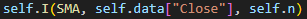
\includegraphics[width=110mm]{fig/I_SMA.png}
    \caption{インディケータメソッド,SMA,self.data}
    \label{fig:ISMA}
   \end{figure}

   \begin{figure}[H]
       \centering
       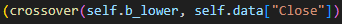
\includegraphics[width=110mm]{fig/crossover.png}
       \caption{クロスオーバーメソッド}
       \label{fig:cros}
      \end{figure}
      \begin{figure}[H]
        \centering
        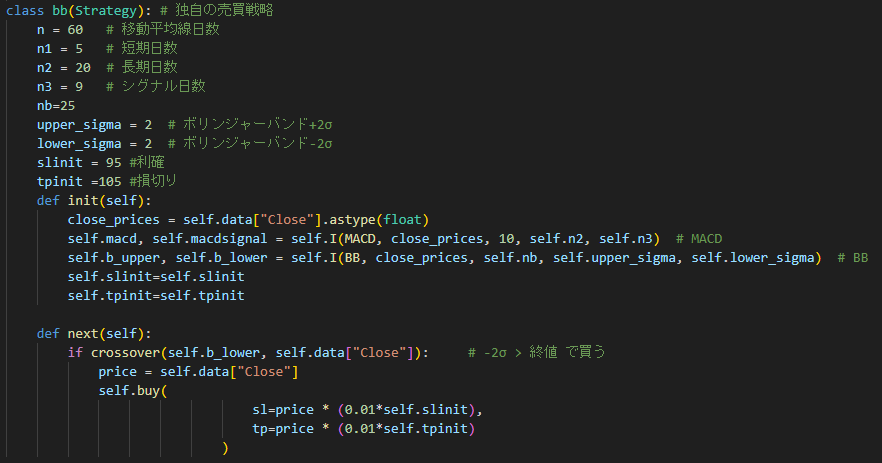
\includegraphics[width=150mm]{fig/strategy.png}
        \caption{売買戦略}
        \label{fig:strat}
       \end{figure}
    

   図\ref{fig:databt}について説明する.\(s\_code\)は銘柄コードを格納しており,dfは独自の\(get\_stock\_data\_from\_file()\)から取得した株価データを格納している.$data$は取得した株価データの2013年1月1日から
   2022年12月31日までの株価データを保持している.
   
   $bt$はBactestingのBacktestクラスを用いてバックテストを初期化する.ここで使用しているのは先ほど説明した$data$,図\ref{fig:strat}で説明した戦略と取引をクローズ時に行うかどうかの設定
   の\(trade\_on\_close\)で,Trueの場合はクローズ時に取引が行われる.

   $result$は$optimize$メソッドで$bt$を最適化している.ここで最適化するパラメータは\(slinit\)と\(tpinit\)で,\(slinit\)は90から100まで1単位,\(tpinit\)は101から110まで1単位で試行する.
   このとき\( Return[\%]\),つまり利益率を最大化するように設定する.
   \begin{figure}[H]
    \centering
    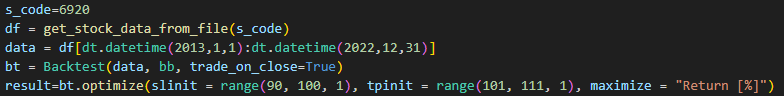
\includegraphics[width=150mm]{fig/data_bt_result.png}
    \caption{バックテスト}
    \label{fig:databt}
   \end{figure}
   図\ref{fig:resbt}に付いて説明する.この図はバックテストを行って最適化実行時の結果である.pandas.DataFrame型のオブジェクトである.ここでは本研究で使用する実行結果のデータは,以下の通りである.
   \begin{description}
    \item[Return[\%]]:10年間の利益率
    \item [\# Trade]:10年間の取引数
    \item [Win Rate[\%]]:10年間の勝率
   \end{description}
   \item [datetime]:datetimeは日時に関するデータを操作するためのクラスを提供している\cite{datetime}.図\ref{fig:datetest}と図\ref{fig:dateres}に簡単な使用例と実行結果を示す.$datetime.now()$メソッドを使って,現在の日付と時刻と取得し,$current\_datetime$に格納している.そのあと$print()$関数で結果を出力する.
  実行結果は図\ref{fig:dateres}のようになる.





  
   
  \item [pandas]:pandasはデータを簡単かつ直感的に扱えるように設計されたデータ構造を提供している\cite{pandas}.
  図\ref{fig:pdtest}と図\ref{fig:pdres}に簡単な使用例と実行結果を示す.辞書型(dictionary)としてデータを定義する.キーとして'Name','Age','City'があり,それぞれのキーに対応する値がリストとして格納されている.
  辞書型のデータを用いてPandasのDataFrameを作成する.DataFrameは表形式のデータ構造で,ここでは'Name','Age','City'の列を持つ3つの行が作成される.そのあと$print()$関数で結果を出力する.実行結果は図\ref{fig:pdres}のようになる.

  \item [numpy]:numPy は,Python を使用した科学技術コンピューティング用のライブラリである\cite{numpy}.図\ref{fig:nptest}と図\ref{fig:npres}に簡単な使用例と実行結果を示す.
  NumPyのarray関数を用いて与えられたリスト$[[1, 2, 3], [4, 5, 6]]$より2次元のNumPy配列を作成する.そのあと$print()$関数で結果を出力する.実行結果は図\ref{fig:npres}のようになる.
  \begin{figure}[H]
    \centering
    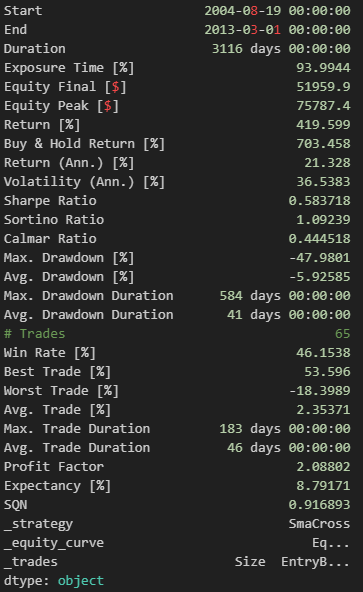
\includegraphics[width=100mm]{fig/bt_res.png}
    \caption{バックテスト実行時の結果}
    \label{fig:resbt}
   \end{figure}

   \begin{figure}[H]
    \centering
    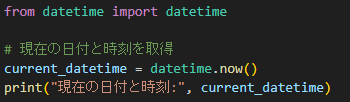
\includegraphics[width=110mm]{fig/datetime_test.png}
    \caption{datetimeの使用例}
    \label{fig:datetest}
   \end{figure}
  
   \begin{figure}[H]
    \centering
    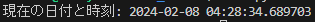
\includegraphics[width=110mm]{fig/datetime_res.png}
    \caption{図\ref{fig:datetest}実行時の結果}
    \label{fig:dateres}
   \end{figure}
  %%%%%%%%%%%%%%%%%%%%%%%%%%%%%%%%%%%%%%%%%%%%%%%%%%%
  
  \begin{figure}[H]
    \centering
    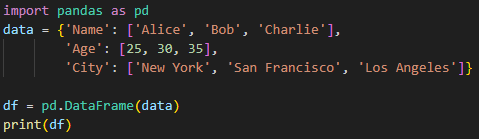
\includegraphics[width=110mm]{fig/pandas_test.png}
    \caption{pandasの使用例}
    \label{fig:pdtest}
   \end{figure}
  
   \begin{figure}[H]
    \centering
    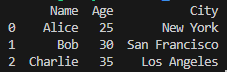
\includegraphics[width=80mm]{fig/pandas_res.png}
    \caption{図\ref{fig:pdtest}実行時の結果}
    \label{fig:pdres}
   \end{figure}

   \begin{figure}[H]
    \centering
    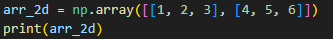
\includegraphics[width=110mm]{fig/np_test.png}
    \caption{numpyの使用例}
    \label{fig:nptest}
   \end{figure}

   \begin{figure}[H]
    \centering
    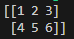
\includegraphics[width=30mm]{fig/np_res.png}
    \caption{図\ref{fig:nptest}実行時の結果}
    \label{fig:npres}
   \end{figure}
  \item [talib]:talibは金融取引で使われている指標のライブラリを提供している\cite{talib}.図\ref{fig:talibtest}と図\ref{fig:talibres}に簡単な使用例と実行結果を示す.
NumPyのrandom関数を用いて,0から1までのランダムな数値を100個生成し,それぞれに100を掛けて仮想の株価データを制作する.Ta-LibのSMA関数を用いて,与えられた株価データに対して20期間の単純移動平均を計算する.そのあと$print()$関数で結果を出力する.
実行結果は図\ref{fig:talibtest}のようになる.


  \item [matplotlib]:matplotlibはアニメーションやグラフを作成するために使われるライブラリである\cite{matplotlib}.図\ref{fig:plttest}と図\ref{fig:pltres}に簡単な使用例と実行結果を示す.
  NumPyのlinspace関数を用いて,0から10までの範囲を100点で均等に区切ったデータを生成する.NumPyのsin関数を用いて,各$x$に対する$sin(x)$の値を計算する.$plt.plot()$メソッドで折れ線グラフをプロットする.
  $plt.title()$メソッドでグラフにタイトルを追加する.$plt.xlabe()$メソッドと$plt.ylabel()$メソッドで x軸とy軸にラベルを追加する.$plt.legend()$メソッドでグラフにを表示する.$plt.show()$メソッドで,
  作成したグラフを表示する.実行結果は図\ref{fig:pltres}のようになる.



 
   %%%%%%%%%%%%%%%%%%%%%%%%%%%%%%%%%%%%%%%%%%%%%%%
 
   %%%%%%%%%%%%%%%%%%%%%%%%%%%%%%%%%%%%%%%%%%%%%

%%%%%%%%%%%%%%%%%%%%%%%%%%%%%%%%%%%%%%%%%%%%%%%%%%
  \begin{figure}[H]
    \centering
    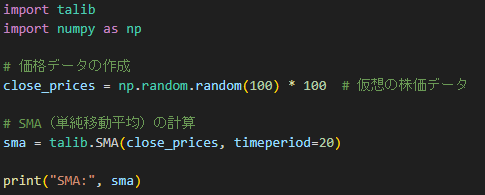
\includegraphics[width=110mm]{fig/talib_test.png}
    \caption{talibの使用例}
    \label{fig:talibtest}
   \end{figure}

   \begin{figure}[H]
    \centering
    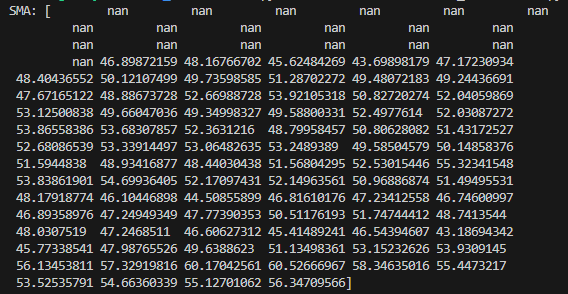
\includegraphics[width=110mm]{fig/talib_res.png}
    \caption{図\ref{fig:talibtest}実行時の結果}
    \label{fig:talibres}
   \end{figure}
   %%%%%%%%%%%%%%%%%%%%%%%%%%%%%%%%%%%%%%%%%%%%%%%%%%
  \begin{figure}[H]
    \centering
    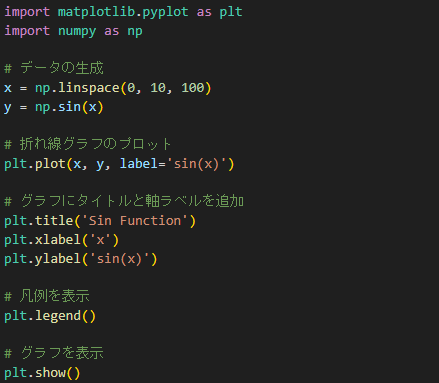
\includegraphics[width=110mm]{fig/plt_test.png}
    \caption{matplotlibの使用例}
    \label{fig:plttest}
   \end{figure}

   \begin{figure}[H]
    \centering
    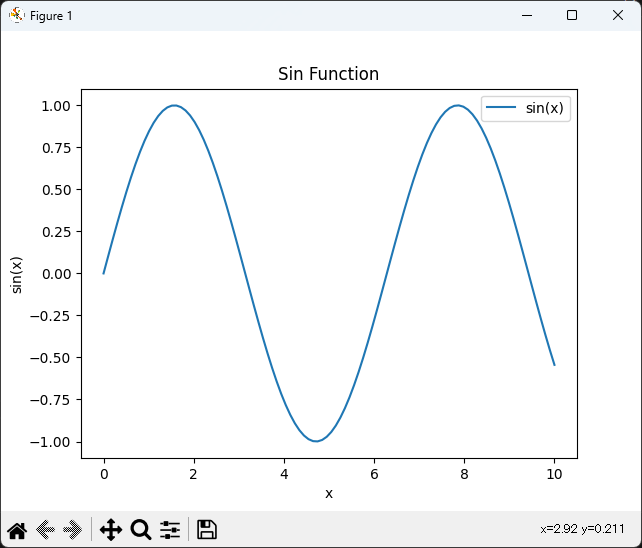
\includegraphics[width=110mm]{fig/plt_res.png}
    \caption{図\ref{fig:plttest}実行時の結果}
    \label{fig:pltres}
   \end{figure}
   %%%%%%%%%%%%%%%%%%%%%%%%%%%%%%%%%%%%%%%%%%%%%%%%%%
\end{description}


\newpage